\section{MAESTRO Architecture}

\subsection{MAESTRO Directory Structure}

\begin{figure}[h]
\centering
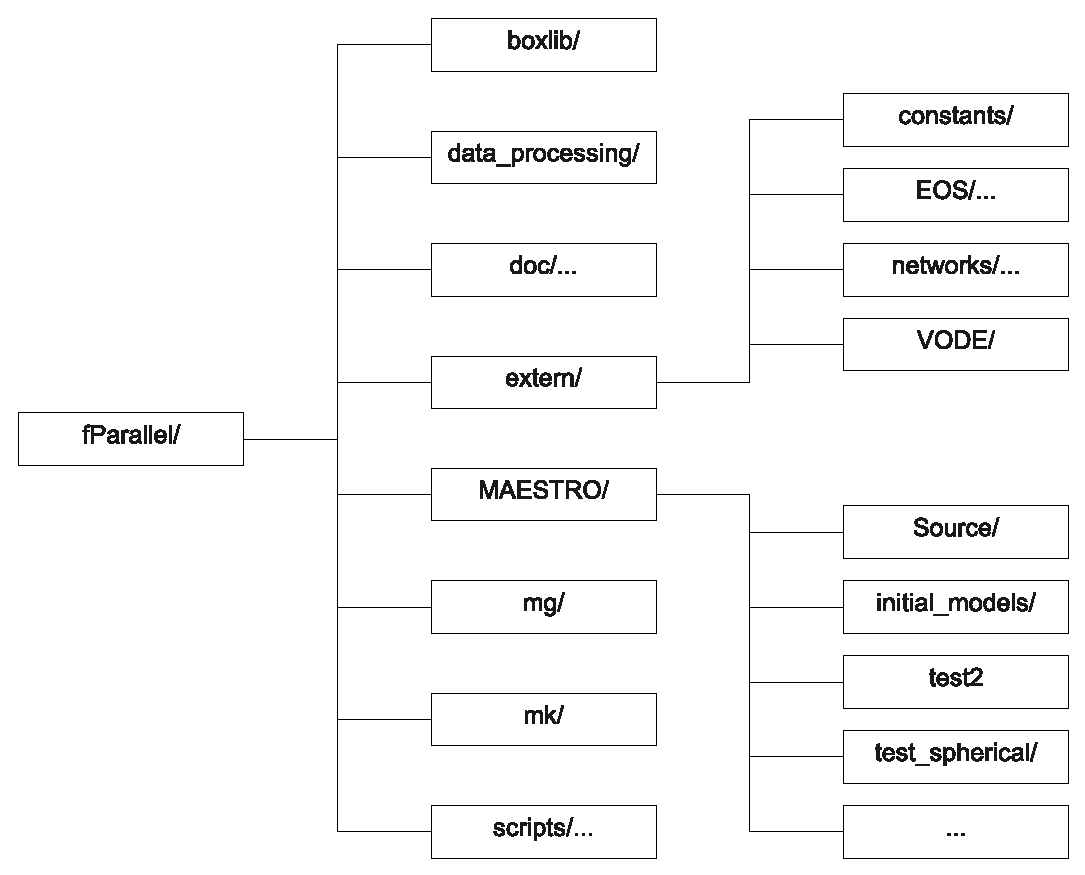
\includegraphics[width=5.0in]{\archfigpath/maestro_directory2}
\caption{The basic MAESTRO directory structure}
\end{figure}

All the files needed to build MAESTRO are contained in the {\tt
fParallel} directory structure.  Briefly, the sub-directories
are:
\begin{itemize}
\item {\tt boxlib/} 

 boxlib is a library for describing meshes consisting of a union
 of boxes.  The boxlib modules define the basic datatypes used
 in MAESTRO.

\item {\tt data\_processing/}

 Simple Fortran-based analysis routines (e.g.\ extract a line from a
 multidimensional dataset) that operate on boxlib plotfiles.

\item {\tt doc/}

 Documentation describing the basic algorithm.

\item {\tt extern/}

 External modules, like ODE integrators, equations of state, reaction
 networks

\item {\tt MAESTRO/}

 The main MAESTRO algorithm files.  Here you will find the main driver,
 the advection routines, etc.

 Important directories under {\tt MAESTRO/} include:

 \begin{itemize}

 \item {\tt initial\_models}

   Several sub-directories containing routines to generate
   1D initial conditions in hydrostatic equilibrium for 
   mapping onto the MAESTRO grid.

 \item problem directories: {\tt test}, {\tt test2}, {\tt
   test\_spherical}, $\ldots$

   Each problem in MAESTRO gets it own subdirectory.  The {\tt
   GNUmakefile} includes the instructions on how to build the
   executable, including what modules in {\tt extern} are used.

   Any file that you place in a sub-directory here takes 
   precedence over a file of the same name in {\tt MAESTRO/}.
   This allows problems to have custom versions of the main
   MAESTRO routines (e.g.\ initial conditions via {\tt initdata.f90}.

 \end{itemize}

\item {\tt mg/}

  The multigrid solver.

\item {\tt mk/}

  The generic Makefiles that store the compilation flags for
  various platforms.

\item {\tt scripts/}

  Some simple scripts that are useful for building, running,
  maintaining MAESTRO.

\end{itemize}



\subsection{BoxLib Data Structures}

\subsubsection{\boxtype}

A \boxtype\ is simply a rectangular domain in space.  Note that boxes
do not hold the state data themselves.  The datatype for a
\boxtype\ is
\begin{verbatim}
  type box
     integer :: dim  = 0
     integer :: lo(MAX_SPACEDIM) =  Huge(1)
     integer :: hi(MAX_SPACEDIM) = -Huge(1)
  end type box
\end{verbatim}

\noindent Here:
\begin{itemize}
\item {\tt dim} is the dimensionality of the data
\item {\tt lo} is the index of the lower bound of the box
\item {\tt hi} is the index of the upper bound of the box
\end{itemize}


\begin{figure}[h]
\centering
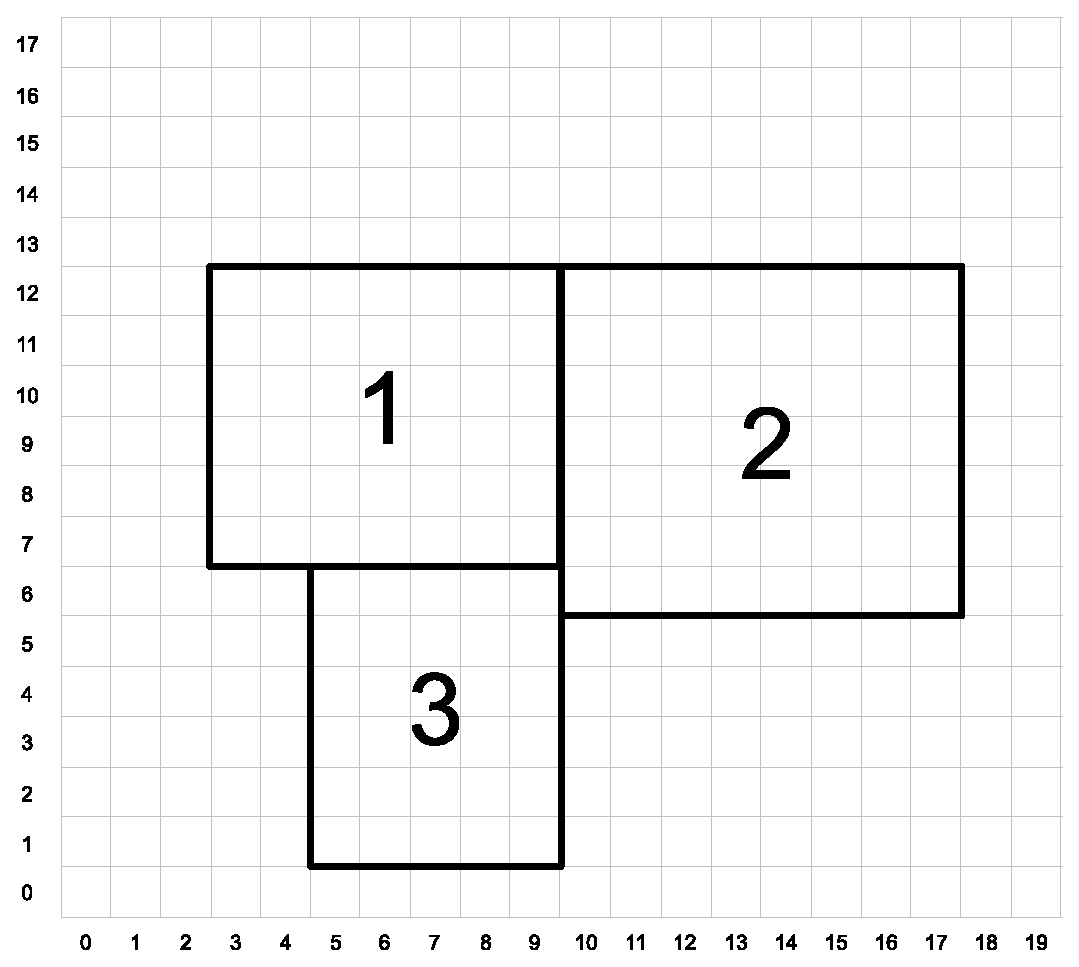
\includegraphics[width=4.0in]{\archfigpath/index_grid2}
\caption{\label{fig:boxes} Three boxes that comprise a single level.
At this resolution, the domain is 20$\times$18 zones.}
\end{figure}


The computational domain is divided into boxes.  The collection of
boxes with the same resolution comprise a level.
Figure~\ref{fig:boxes} shows three boxes in the same level of
refinement.  The position of the boxes is with respect to a global
index space at that level.  For example, box 1 in the figure has {\tt
  lo} = (3,7) and {\tt hi} = (9,12).


\subsubsection{\fab}

A \fab\ is a ``Fortran Array Box''.  It contains the state data in a
multidimensional array and several \boxtype-types to describe where in
index-space it lives.  The datatype of a \fab\ is
\begin{verbatim}
  type fab
     integer   :: dim = 0
     type(box) :: bx
     type(box) :: pbx
     type(box) :: ibx
     integer   :: nc = 1
     real(kind = dp_t), pointer, dimension(:,:,:,:) :: p => Null()
  end type fab
\end{verbatim}
 
\noindent Here:
\begin{itemize}
\item {\tt dim} is the dimensionality of the data
\item {\tt bx} is a \boxtype\ describing where the data in this
  \fab\ is defined.
\item {\tt pbx} is a \boxtype\ that extends {\tt bx} to include
  any ghostcells
\item {\tt ibx}
\item {\tt nc} is the number of components (how many variables at  
  each grid location).
\item {\tt p} is a pointer to the data.
\end{itemize}

Note that alternate datatypes exist for data that is not
double-precision.

Also note that all state data is stored in a four-dimensional array,
{\tt (nx,ny,nz,nc)} in size, regardless of the dimensionality of the
problem.  For 2D problems, {\tt nz=1}.

\subsubsection{\multifab}

A \multifab\ is a collection of \fab s at the same level of
refinement.

\subsubsection{\boxarray}

\subsubsection{\mlboxarray}

\subsubsection{\mllayout}

\subsubsection{\bctower}


\subsection{Example: Accessing State Data}

In MAESTRO, the state data is stored in a multifab array (the array
index refers to the AMR level).  A typical way to extract the state data
array looks like:

\begin{verbatim}
  subroutine example(s,dx,dt)

    use bl_types
    use multifab_module
    use geometry, only: dm, nlevs
    use variables, only: rho_comp
\end{verbatim}

\noindent Here, the {\tt bl\_types} and {\tt multifab\_types} modules
bring in the basic boxlib data types Specifically, here, {\tt
bl\_types} defines {\tt dp\_t} which is the {\tt kind} used for
declaring double precision data, and {\tt multifab\_module} defines
the \multifab\ data type.  The {\tt geometry} module is a MAESTRO
module that provides the dimensionality ({\tt dm}) and the number of 
levels ({\tt nlevs}).  The {\tt variables} module is a MAESTRO
module that provides integer keys for indexing the state arrays.  In
this case the integer {\tt rho\_comp} refers to the location in the
state array corresponding to density.

\begin{verbatim}
    type(multifab) , intent(inout) :: s(:)
    real(kind=dp_t), intent(in   ) :: dx(:,:),dt
\end{verbatim}

\noindent Next we declare the subroutine arguments.  Here, {\tt s(:)}
is our \multifab\ array that holds the state data.  The array index
in {\tt s} refers to the AMR level.

\begin{verbatim}
    ! Local variables
    real(kind=dp_t), pointer :: sp(:,:,:,:)
    integer :: i,n,ng_sp
    integer :: lo(dm),hi(dm)
\end{verbatim}

\noindent Amongst the local variables we define here are a pointer,
{\tt sp}, that will point to a single \fab\ from the
\multifab\ {\tt s}.

\begin{verbatim}
    ng_sp = s(1)%ng
\end{verbatim}

\noindent Here we get the number of ghostcells for this particular
\multifab.  This will be needed to access the data stored in the
\fab s.  Note that all levels in a \multifab\ will have the same
number of ghostcells, so we can use {\tt s(1)} here.

\begin{verbatim}
    do n=1,nlevs
       do i = 1, s(n)%nboxes
\end{verbatim}

\noindent To access the data, we loop over all the levels, and
all the boxes in the given level.  {\tt s(n)\%nboxes} is simply
the number of boxes in level {\tt n}.

\begin{verbatim}
          if ( multifab_remote(s(n), i) ) cycle
          sp => dataptr(s(n), i)
          lo =  lwb(get_box(s(n), i))
          hi =  upb(get_box(s(n), i))
\end{verbatim}

\noindent For parallel runs, there is no guarantee that the particular
box is on the current processor.  The function {\tt multifab\_remote}
returns {\tt .true.} if the box is off-processor, in which case, we 
simply skip to the next box.

The actual data array is accessed through the {\tt dataptr} function,
which takes a \multifab\ (in this case, {\tt s(n)}) and the index of
the \boxtype\ ({\tt i}) we want.  {\tt sp} is always four-dimensional:
3 spatial dimensions and 1 for the components.

Finally, the index bounds of the box (just the data, not the ghostcells) are 
stored in the {\tt dm}-dimensional arrays {\tt lo} and {\tt hi}

\begin{verbatim}
          select case (dm)
          case (2)
             call example_2d(sp(:,:,1,rho_comp),ng_sp,lo,hi,dx(n,:),dt)
          case (3)
             call example_3d(sp(:,:,:,rho_comp),ng_sp,lo,hi,dx(n,:),dt)
          end select
       end do

    end do

  end subroutine example
\end{verbatim}

\noindent Finally, in this example, we call either the function
{\tt example\_2d} for two-dimensional data or {\tt example\_3d}
for three-dimensional data.  Note that in the two-dimensional
case, we index the data as {\tt sp(:,:,1,rho\_comp)}.  Here a
`{\tt 1}' is used as the `z'-coordinate spatial index, since this
is a 2D problem, and the density component of the state is selected
(using the integer key {\tt rho\_comp}).

This routine will be supplimented with {\tt example\_2d} and {\tt
example\_3d}, which actually operate on the data.  The form of 
these functions is:

\begin{verbatim}
  subroutine example_2d(density,ng_sp,lo,hi,dx,dt)

    use bl_constants_module
    use probin_module, only: prob_lo

    integer        , intent(in) :: lo(:),hi(:), ng_sp
    real(kind=dp_t), intent(in) :: density(lo(1)-ng_sp:,lo(2)-ng_sp:)
    real(kind=dp_t), intent(in) :: dx(:),dt

    integer         :: i, j
    real(kind=dp_t) :: x, y

    do j = lo(2), hi(2)
       y = prob_lo(2) + (dble(j) + HALF)*dx(2)

       do i = lo(1), hi(1)
          x = prob_lo(1) + (dble(i) + HALF)*dx(1)

          ! operate on density(i,j)

       enddo
    end do

  end subroutine mk_sponge_2d
\end{verbatim}

\noindent In this function, the bounds of the {\tt density} array
take into account the {\tt ng\_sp} ghostcells.  The {\tt j} and {\tt i}
loops loop over all the valid zones.  Coordinate information is 
computed from {\tt dx} and {\tt prob\_lo} which is the physical
lower bound of the domain.  {\tt bl\_constants\_module} declares
useful double-precision constants, like {\tt HALF} (0.5).

The three-dimensional case is similar, with the {\tt density} array
declared as 
\begin{verbatim}
  density(lo(1)-ng_sp:,lo(2)-ng_sp:,lo(3)-ng_sp)
\end{verbatim}
and an additional loop over the `z' coordinate (from {\tt lo(3)} to
{\tt hi(3)}).

\subsection{Working with Multifabs}


\subsection{Filling Ghostcells}


\subsection{Boundary Conditions}



\section{Adding A Problem}



